\documentclass{llncs}

\usepackage{proof}
\usepackage{amssymb}
\usepackage{amsmath}
\usepackage{graphicx}
\usepackage{skak} % for the \qside
\usepackage{mathpartir}
\usepackage{array}
\usepackage{url}

\newcommand{\fun}[1]{\mbox{\textbf{#1}}}
\newcommand{\lb}[1]{#1_{\downarrow}}
\newcommand{\ub}[1]{#1_{\uparrow}}
\newcommand{\varset}[1]{\mbox{$\cal{#1}$}}

\sloppy


\begin{document}

\title {Range Analysis of Whole Programs}

\author{Victor Sperle Campos, Igor Rafael, Douglas do Couto Teixeira,
Fernando Magno Quint\~{a}o Pereira}

\institute{UFMG -- 6627 Ant\^{o}nio Carlos Av, 31.270-010, Belo Horizonte, Brazil
\email{\{victorsc,igor.rafael,douglas,fernando\}@dcc.ufmg.br}
}


\maketitle

%mmmmmmmmmmmmmmmmmmmmmmmmmmmmmmmmmmmmmmmmmmmmmmmmmmmmmmmmmmmmmmmmmmmmmmmmmmmmmm
\begin{abstract}
This paper describes an inter-procedural range analysis algorithm that scales
up to programs with millions of assembly instructions.
Contrary to many previous techniques, we handle comparisons between variables
without resorting to relational lattices or expensive algorithms.
We achieve path sensitiveness by using Bodik's Extended Static Single
Assignment form as the intermediate representation.
We show that by processing the strongly connected components that constitute
the graph of dependences between variables in topological order we not only
gain in time, but also in precision.
We have implemented our technique in LLVM, an industrial strength compiler,
and have been able to process over 4 million assembly instructions in a
few seconds.
\end{abstract}

\section{Introduction}
\label{sec:intro}

% The context: why range analysis is necessary.
The analysis of integer variables on the interval lattice has been the
canonical example of abstract interpretation since its introduction in
Cousot and Cousot's seminal paper~\cite{Cousot77}.
Compilers use range analysis to infer the possible values that discrete
variables may assume during program execution.
This analysis has many uses.
For instance, it allows the optimizing compiler to remove from the program text
redundant overflow tests~\cite{Sol11} and unnecessary array bound
checks~\cite{Bodik00}.
Additionally, range analysis is essential not only to the bitwidth aware
register allocator~\cite{Barik06,Tallam03}, but also to more traditional
allocators that handle registers of different
sizes~\cite{Kong98,Pereira08,Scholz02}.
Finally, range analysis has also seen use in the static prediction of
branches~\cite{Patterson95}, to detect buffer overflow
vulnerabilities~\cite{Simon08,Wagner00}, to find the trip count of
loops~\cite{Lokuciejewski09}
and even in the synthesis of hardware~\cite{Cong05,Mahlke01}.

% The problem: few implementations, not extensive experimental reports.
Given this great importance, it comes as no surprise that the compiler
literature is rich in works describing in details algorithmic variations of
range analyses~\cite{Gawlitza09,Mahlke01,Stephenson00,Su05}.
On the other hand, none of these authors provide experimental evidence that
their approaches are able to deal with very large programs.
There are researchers who have implemented range analyses that scale up to
large programs~\cite{Blanchet03,Venet04}; nevertheless, because the
algorithm itself is not the main focus of their works, they neither give
details about their design choices nor provide experimental data about it.
This scenario was recently changed by Oh {\em et al.}~\cite{Oh12}, who
introduced an abstract interpretation framework which processes programs with
hundreds of thousands of lines of code.
Nevertheless, Oh {\em et al.} have designed a very simple range analysis,
which does not handle comparisons between variables, for instance.
They also do not discuss the precision of their implementation, but only its
runtime.

% Our contribution.
In this paper we provide a complete description of a range analysis algorithm,
and show extensive experimental data that justifies our engineering choices.
Our first algorithmic contribution on top of previous works is a three-phases
approach to handle comparisons between variables without resorting to any
exponential time technique.
The few publicly available implementations of range analyses that we are
aware of, such as those in FLEX~\footnote{The MIT's FLEX/Harpoon compiler
provides an implementation of Stephenson's algorithm~\cite{Stephenson00}, and
is available at \texttt{http://flex.cscott.net/Harpoon/}.} and
gcc~\footnote{Gcc's VRP pass implements a variant of Patterson's
algorithm~\cite{Patterson95}.} only deal with comparisons between variables and
constants.
Even theoretical works, such as Su and Wagner's~\cite{Su05} or Gawlitza
{\em et al.}'s~\cite{Gawlitza09} suffer from this limitation.
This deficiency is one of the reasons explaining why none of these works has
made their way into industrial-strength compilers.
Two other insights allow our implementation to scale up to very large
programs.
We use Bodik's Extended Static Single Assignment (e-SSA) form~\cite{Bodik00} to
perform range analysis sparsely.
This program representation ensures that the interval associated with
a variable is constant along its entire live range, and allows us to compute
path-sensitive results.
Finally, we process the strongly connected components that underline our
constraint system in topological ordering.
It is well-know that this technique is essential to speedup constraint solving
algorithms~\cite[Sec 6.3]{Nielson99}; however, we show that a careful
propagation of information along strong components not only gives us speed, but
also improves the precision of our results.

% The history of our contribution.
This work concludes a two years long effort to produce a solid and scalable
implementation of range analysis.
Our first endeavor to implement such an algorithm was based on Su and
Wagner's constraint system, which can be solved exactly in polynomial
time~\cite{Su04,Su05}.
However, although we could use their formula to handle a subset of C-like
constructs, their description of how to deal with loops was
``not very explicit"~\cite[p.422]{Gawlitza09}.
Thus, in order to solve loops we adopted Gawlitza
{\em et al.}'s~\cite{Gawlitza09} approach.
This technique uses the Bellman-Ford algorithm to detect increasing or
decreasing cycles in the constraint system, and then saturates these cycles
via a simple widening operator.
A detailed description of our implementation has been published by
Couto and Pereira~\cite{Couto11}.
Nevertheless, the inability to handle comparisons between variables, and the
cubic complexity of the Bellman-Ford method eventually lead us to seek
alternative solutions to range analysis.
This quest reached a pinnacle in the present work.

% Our experimental numbers.
We have implemented our algorithm in the LLVM compiler~\cite{Lattner04}, and
have used it to analyze a test suite with 1.4 million lines of C code.
In Section~\ref{sec:exp} we provide empirical evidence showing that our
implementation is fast: it analyzes the gcc source code in 4 seconds, for
instance.
It is also precise: our results are similar to Stephenson
{\em et al}'s~\cite{Stephenson00}, even though, contrary to them, we do not
assume that the program is correct.
Furthermore, we have been able to find tight bounds to many of the examples
used by Costan {\em et al.}~\cite{Costan05} and Lakhdar
{\em et al.}~\cite{Lakhdar11}, who rely on much more costly methods.

% The rest of this paper.

\section{Background}
\label{sec:bck}

% Define the lattice, the constraints and the valuation I.
Following Gawlitza {\em et al.}'s notation, we shall be performing arithmetic
operations over the complete lattice
$\cal{Z} = \mathbb{Z} \cup \{-\infty, +\infty\}$, where the ordering is
naturally given by $-\infty < \ldots < -2 < -1 < 0 < 1 < 2 < \ldots +\infty$.
For any $x > -\infty$ we define:

\begin{tabular}{lcl}
$x + \infty = \infty, x \neq -\infty$ & \mbox{\hspace{0.1cm}} & $x - \infty = - \infty, x \neq +\infty$ \\
$x \times \infty = \infty$ if $x > 0$ & & $x \times \infty = -\infty$ if $x < 0$ \\
$0 \times \infty = 0$ & & $(-\infty) \times \infty = \ $ not defined $$ \\
\end{tabular}

From the lattice $\varset{Z}$ we define the product lattice
$\varset{Z}^2$, which is partially ordered by the subset relation
$\sqsubseteq$.
$\varset{Z}^2$ is defined as follows:

\begin{equation*}
\varset{Z}^2 = \emptyset \cup \{[z_1, z_2] | \ z_1,z_2 \in \varset{Z},
\ z_1 \leq z_2, \  -\infty < z_2 \}
\end{equation*}

Given an interval $\iota = [l, u]$, we let $\lb{\iota} = l$, and
$\ub{\iota} = u$.
We let \varset{V} be a set of constraint variables, and
$I: \varset{V} \mapsto \varset{Z}^2$ a
mapping from these variables to intervals in $\varset{Z}^2$.
Our objective is to solve a constraint system $C$, formed by instances of the
six different types of constraints seen in Figure~\ref{fig:eval_function}
(left).
Figure~\ref{fig:eval_function} (right) defines a valuation function $e$ that
computes $Y = f(\ldots)$, given I.
Armed with these concepts, we define the range analysis problem as follows:

\begin{definition}
\label{def:rcp}
\textsc{Range Analysis Problem} \\
\textbf{Input:} a set $C$ of constraints ranging over a set \varset{V} of
variables. \\
\textbf{Output:} a mapping I such that, for any variable
$V \in \varset{V}$, e(V) = I[V].
\end{definition}

\begin{figure}[hbt]
\begin{small}
\begin{eqnarray*}
\begin{array}{r@{\hspace{0.5cm}}c}
Y = [l, u]
&
e(Y) = [l, u]
\\
\\
Y = \phi (X_1, X_2)
&
\inferrule{I[X_1]=[l_1, u_1] \\ I[X_2]=[l_2, u_2]}
{e(Y) = [\mbox{min}(l_1, l_2), \mbox{max}(u_1, u_2)]}
\\
\\
Y = X_1 + X_2
&
\inferrule{I[X_1]=[l_1, u_1] \\ I[X_2]=[l_2, u_2]}
{e(Y) = [l_1 + l_2, u_1 + u_2]}
\\
\\
Y = X_1 \times X_2
&
\inferrule{I[X_1]=[l_1, u_1] \\ I[X_2]=[l_2, u_2] \\ L = \{l_1l_2, l_1u_2, u_1l_2, u_1u_2\}}
{e(Y) = [\mbox{min}(L), \mbox{max}(L)]}
\\
\\
Y = aX + b
&
\inferrule{I[X]=[l, u] \\ k_l = al + b \\ k_u = au + b}
{e(Y) = [\mbox{min}(k_l, k_u), \mbox{max}(k_l, k_u)]}
\\
\\
Y = X \sqcap [l', u']
&
\inferrule{I[X]=[l, u]}
{e(Y) \leftarrow [\mbox{max}(l, l'), \mbox{min}(u, u')]}
\end{array}
\end{eqnarray*}
\caption{\label{fig:eval_function}
The constraint system that produces instances of the range analysis problem.}
\end{small}
\end{figure}

We will use the program in Figure~\ref{fig:ex1}(a) as the running example
to illustrate our range analysis.
Figure~\ref{fig:ex1}(b) shows the same program in SSA form~\cite{Cytron91},
and Figure~\ref{fig:ex1}(c) outlines the constraints that we extract from this
program.
There is a clear correspondence between instructions and constraints.
A possible solution to the range analysis problem, as obtained via the
techniques that we will introduce in Section~\ref{sec:algo}, is given in
Figure~\ref{fig:ex1}(d).
The SSA form, so conspicuous in modern compilers, leads to a very conservative
solution.
As we will see shortly, we can improve this solution substantially by using
a more sophisticated program representation -- the e-SSA form.

\begin{figure}[t!]
\begin{center}
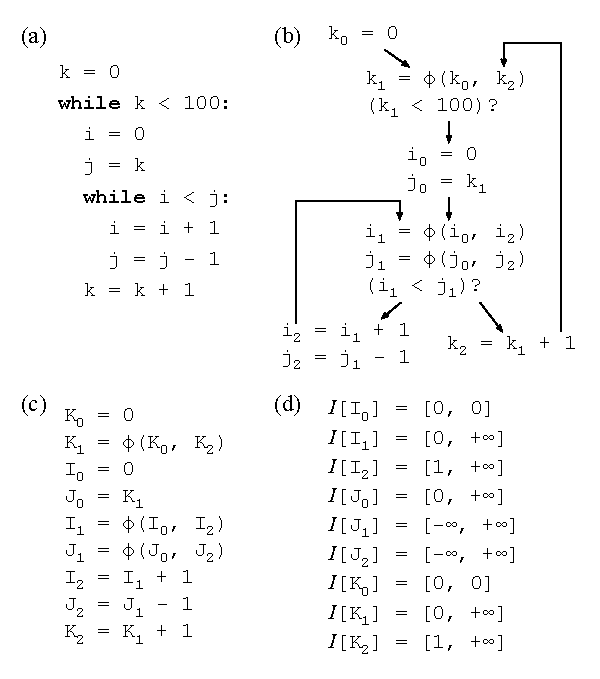
\includegraphics[width=0.7\textwidth]{images/ex1}
\end{center}
\caption{\label{fig:ex1}
(a) Example program.
(b) Control Flow Graph (CFG) in SSA form.
(c) Constraints that we extract from the program.
(d) A possible solution to the range analysis problem.}
\end{figure}

\section{Our Design of a Range Analysis Algorithm}
\label{sec:algo}

% Program representation
% Extracting constraints
% Building the Constraint graph (pseudo-edges)
% Macro algorithm
% Micro algorithm

In this section we explain the algorithm that we use to solve the range
analysis problem for an entire program.
This algorithm involves a number of steps.
First, we convert the program to a suitable intermediate representation that
makes it easier to extract constraint.
From these constraints, we build a dependence graph that allows us to do
range analysis sparsely.
Finally, we solve the constraints applying different fix-point iterators on
this dependence graph.
Figure~\ref{fig:algorithm} gives a global view of this algorithm.
Some of the steps in the algorithm are optional.
They improve the precision of the range analysis, at the expenses of a longer
running time.

\begin{figure}[t!]
\begin{center}
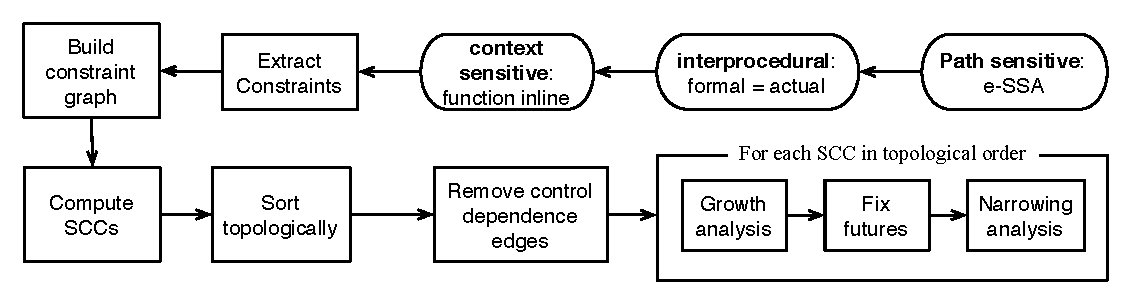
\includegraphics[width=0.8\textwidth]{images/algorithm}
\end{center}
\caption{\label{fig:algorithm}
Our algorithm to solve the range analysis problem.
Rounded boxes are optional steps.}
\end{figure}

\subsection{Choosing a Program Representation}
\label{sub:rep}

The solution that we found to the range analysis problem in Figure~\ref{fig:ex1}
is imprecise because we did not take conditional tests into considerations.
Branches gives us information about the ranges that some variables assume, but
only at {\em specific} program points.
For instance, given a test such as $(k_1 < 100)?$ in  Figure~\ref{fig:ex1}(b),
we know that $I[k_1] \sqsubseteq [-\infty, 99]$ whenever the condition is true.
In order to encode this information, we might split the live range of $k_1$
right after the branching point; thus, creating two new variables, one at the
path where the condition is true, and another where it is false.
There is a program representation, introduced by Bodik
{\em et al.}~\cite{Bodik00}, that performs this live range splitting:
the {\em Extended Static Single Assignment} form, or e-SSA for short.
In this paper, we have experimented with two different flavors of e-SSA form,
which we call {\em standard} and {\em non-pruned}.

We will show first how we convert a program into standard e-SSA form.
Let $(v < c)?$ be a conditional test, and let $l_t$ and $l_f$ be labels in
the program, such that $l_t$ is the target of the test if the condition is true,
and let $l_f$ is the target when the condition is false.
If $l_t$ dominates any use of $v$, then we insert at $l_f$ a copy
$v_f = v \sqcap [-\infty, c-1]$, where $v_f$ is a fresh name.
We then rename every use of $v$ that is dominated by $l_f$ to $v_f$.
Dually, if $l_t$ dominates any use of $v$, then we insert at $l_t$ a copy
$v_t = v \sqcap [c, +\infty]$, and rename variables accordingly.
If the test uses two variables, e.g., $(v_1 < v_2)?$, then we create
intersections bound to {\em futures}.
We insert, at $l_f$, $v_{1f} = v_1 \sqcap [\fun{ft}(v_2), +\infty]$,
and $v_{2f} = v_2 \sqcap [-\infty, \fun{ft}(v_1) - 1]$.
Similarly, at $l_v$ we insert
$v_{1v} = v_1 \sqcap [-\infty, \fun{ft}(v_2) - 1]$
and $v_{2f} = v_2 \sqcap [\fun{ft}(v_1), +\infty]$.
We use the notation $\fun{ft}(v)$ to denote the {\em future} bounds of a
variable.
As we will show in Section~\ref{sub:micro}, once the growth pattern of $v$ is
known, we can replace $\fun{ft}(v)$ by an actual value.
Once we are done placing copies, we insert $\phi$-functions into the
transformed program to convert it to SSA form.
This last step avoids that two different names given to the same original
variable be simultaneously alive at the program code.
Figure~\ref{fig:ex_standard_eSSA}(a) shows our running example changed into
standard e-SSA form.
The part (b) of this figure shows the solution that we get to this new
program.

\begin{figure}[t!]
\begin{center}
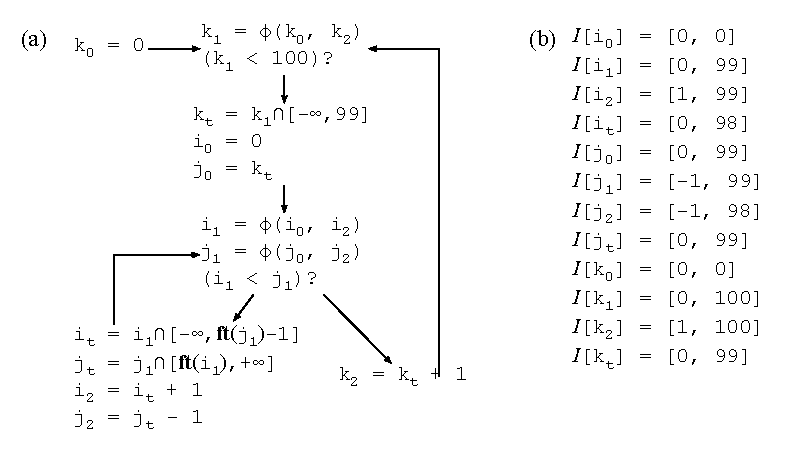
\includegraphics[width=0.9\textwidth]{images/ex_standard_eSSA}
\end{center}
\caption{\label{fig:ex_standard_eSSA}
(a) The control flow graph from Figure~\ref{fig:ex1}(b) converted to standard
e-SSA form.
(b) A solution to the range analysis problem
}
\end{figure}

The standard e-SSA form serves well analysis that need range information
at the use site of variables, such as conditional constant propagation,
redundant code elimination and detection of buffer overflows.
On the other hand, there exist compilation algorithms that require range
information at the whole live range of variables.
Examples of such algorithms include the family of
bitwidth aware register allocators~\cite{Barik06,Pereira08,Tallam03} and
hardware synthesizers~\cite{Cong05,Mahlke01,Stephenson00}.
In order to provide extra precision to these algorithms, we may work with a
non-pruned version of e-SSA form, which we produce by simply inserting copies
after every conditional test, and then reconverting the entire program to
SSA form.
Figure~\ref{fig:ex_non_pruned} illustrates the difference between these two
program representations.
Notice that the non-pruned flavor might introduce dead variables in the
program code, which can be removed by standard dead code elimination.

\begin{figure}[t!]
\begin{center}
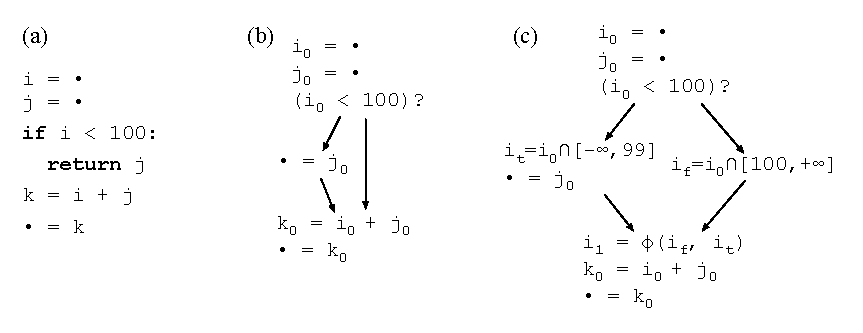
\includegraphics[width=0.9\textwidth]{images/ex_non_pruned}
\end{center}
\caption{\label{fig:ex_non_pruned}
(a) Example program.
(b) Standard e-SSA form.
(c) Non-pruned e-SSA form.}
\end{figure}

\subsection{Extracting Constraints}
\label{sub:constraints}

The constraints in Figure~\ref{fig:eval_function} handles
many different programming instructions.
The $\phi$ assignments, such as $Y = \phi(X_1, X_2)$, represent
the $\phi$-functions typically found in SSA form programs.
As discussed in Section~\ref{sub:rep}, we use intersection
constraints to bound the variables created due to live range splitting
at conditionals.
The widening analysis that we will introduce in Section~\ref{sub:micro}
require monotonic transfer functions.
Many assembly operations, such as modulus or division, do not afford us
this monotonicity.
However, these non-monotonic instructions have a conservative
translation to our constraint system.
Figure~\ref{fig:constraints} shows some examples of constraints that we
derive from typical assembly instructions.

\begin{figure}[t!]\begin{center}
\begin{tabular}{|l@{\hspace{0.2cm}}l@{\hspace{0.3cm}}l|} \hline
\textbf{Description} & \textbf{Operation} & \textbf{Constraint} \\ \hline
Constant & $v = c$ & $V = [c, c]$ \\
Assignment & $v_1 = v_2$ & $V_1 = V_2$ \\
Multiplication & $v_1 = v_2 * c$ & $V_1 = c V_2$ \\
Int. division & $v_1 = v_2 \ / \ v_3$ & $V_1 = V_2$ \\
 & & $V_1 = - V_2$ \\
Modulus & $v_1 = v_2 \ \% \ c$ & $V_1 = [0, c - 1]$ \\
Bitwise and & $v_1 = v_2 \ \& \ c$ & $V_1 = v_2 \sqcap [0, c]$ \\
Bitwise or & $v_1 = v_2 \ | \ v_3$ & $V_1 = V_2 + V_3$ \\
Left shift & $v_1 = v_2 \ \qside \ c$ & $V_1 = 2^c V_2$ \\ \hline
\end{tabular}
\end{center}
\caption{\label{fig:constraints}Example of constraint derivation rules.
We let $c$ denote a positive constant, $\{v, v_1, v_2\}$ are program
variables and $\{V, V_1, V_2\} \subset \cal{V}$.}
\end{figure}

\subsection{The Dependence Graph}
\label{sub:graph}

The main data structure that we use to solve the range analysis problem is
a variation of Ferrante {\em et al.}'s {\em program dependence
graph}~\cite{Ferrante87}.
For each constraint variable $V$ we create a variable node $N_v$.
For each constraint $C$ we create a constraint node $N_c$.
We add an edge from $N_v$ to $N_c$ if the name $V$ is used in $C$.
We add an edge from $N_c$ to $V$ if the constraint $C$ defines the name
$V$.
Figure~\ref{fig:ex_graph} shows the dependence graph that we build for the
e-SSA form program given in Figure~\ref{fig:ex_standard_eSSA}(a).
If $V$ is used by $C$ as the input of a future, then the edge from
$N_v$ to $N_c$ represents what Ferrante {\em et al.} call a {\em control
dependence}~\cite[p.323]{Ferrante87}.
We use dashed lines to represent these edges.
All the other edges denote {\em data dependences}~\cite[p.322]{Ferrante87}.

\begin{figure}[t!]
\begin{center}
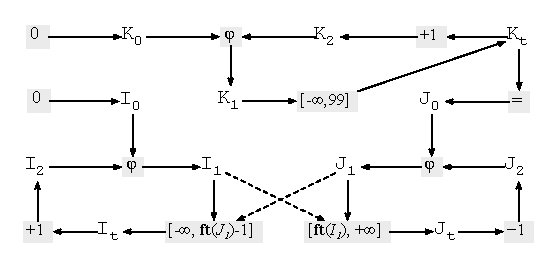
\includegraphics[width=0.7\textwidth]{images/ex_graph}
\end{center}
\caption{\label{fig:ex_graph}
The dependence graph that we build to the program in
Figure~\ref{fig:ex_standard_eSSA}.}
\end{figure}

\subsection{Solving Range Analysis on Strong Components}
\label{sub:macro}

Having built the dependence graph, we proceed to solve the range analysis
problem by finding all the strongly connected components (SCCs) of the
dependence graph, and reducing this graph to a directed acyclic graph.
We perform this last step by collapsing every SCC into a single node.
We then sort the resulting DAG topologically, and apply the analyses from
Section~\ref{sub:micro} on every SSC in topological order.
Once we solve the range analysis problem for a SCC, we propagate the
intervals that we found to the variable nodes at the {\em frontier} of this
SCC.
A variable node $N_v$ is said to be in the frontier of a strongly connected
component $S$ if:
(i) $N_v \notin S$; and
(ii) there exists a variable node $V' \in S$, and a constraint node $N_c$,
such that $V' \leftarrow N_c$, and $N_c \leftarrow V$.
This propagation gives us a very modular algorithm:
when analyzing a strongly connected component $S$ we can rest assured that
any influence that $S$ might suffer from nodes outside it has been already
taken into consideration.

When finding strongly connected components, we take control dependence
edges into consideration.
For instance, in Figure~\ref{fig:ex_graph} the nodes that correspond to the
variables $i_1$, $i_2$, $i_t$, $j_1$, $j_2$ and $j_t$ form a single component.
The dashed edges, which represent control dependences, keep all these variables
connected.
In this way, we ensure that, upon stumbling upon an interval associated with
future bounds, e.g., $\fun{ft}(v)$, either variable $v$ has been solved in a
previous component, or it belongs to the current component.
In the latter case, as we will see soon, we can still take $v$'s interval into
consideration.

\subsection{Finding Ranges: the Micro Algorithm}
\label{sub:micro}

Given a strongly connected component of the dependence graph with $N$ nodes,
we solve the range analysis problem in three-steps:
\begin{enumerate}
\item Run widening analysis: $O(N)$.

\item Fix intersections: $O(N)$.

\item Run narrowing analysis: $O(N^2)$.

\end{enumerate}
However, before we start, we remove control dependence edges from the
strongly connected component, as they have no semantics to our transfer
functions.

\paragraph{Widening Analysis.}

The first step of our algorithm consists in determining the growth behavior of
the interval bound to each constraint variable.
We accomplish this task via Cousot and Cousot's widening
operator~\cite[p.247]{Cousot77}.
The possible behaviors of an interval are:
(i) does not change;
(ii) grows towards $+\infty$;
(iii) grows towards $-\infty$; and
(iv) grows in both directions.
The lattice of abstract states, plus a constraint system that represents our
widening analysis is given in Figure~\ref{fig:growth_analysis}.
Because the lattice has height three, the intervals bound to each variable can
change at most three times.

\begin{figure}[t!]
\begin{center}
\begin{tabular}{c@{\hspace{1.5cm}}c}
\begin{minipage}{2.4cm}
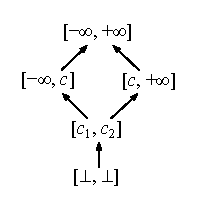
\includegraphics{images/growth_lattice}
\end{minipage}
&
\begin{minipage}{6cm}
\begin{small}
\begin{eqnarray*}
\begin{array}{c}
\inferrule{I[Y] = [\bot, \bot]}{I[Y] \leftarrow e(Y)}
\\
\\
\inferrule{\lb{e(Y)} < \lb{I[Y]} \\ \ub{e(Y)} > \ub{I[Y]}}
{I[Y] \leftarrow [-\infty, +\infty ]}
\\
\\
\inferrule{\lb{e(Y)} < \lb{I[Y]}}
{I[Y] \leftarrow [-\infty, \ub{I[Y]}]}
\\
\\
\inferrule{\ub{e(Y)} > \ub{I[Y]}}
{I[Y] \leftarrow [\lb{I[Y]}, +\infty]}
\end{array}
\end{eqnarray*}
\end{small}
\end{minipage}
\end{tabular}
\end{center}
\caption{\label{fig:growth_analysis}
(Left) The lattice of the widening analysis.
(Right) Cousot and Cousot's widening operator. We evaluate the rules from top 
to bottom, and stop upon finding a pattern matching.}
\end{figure}

\paragraph{Fixing futures.}

The ranges found by the widening analysis tells us which variables have fixed
bounds, independent on the intersections in the constraint system.
Thus, we can use actual limits to replace intersections bounded by futures.
Figure~\ref{fig:fix_intersects} shows the rules to perform these substitutions.
In order to correctly replace a future $\fun{ft}(V)$ that limits a variable
$V'$, we need to have already applied the widening analysis onto $V$.
Had we considered only data dependence edges, then it would be possible
that $V$ be analyzed before $V'$.
However, because of control dependence edges, this case cannot happen.
The control dependence edges ensure that any topological ordering of the
constraint graph either places $N_v$ before $N_{v'}$, or places these nodes
in the same strongly connected component.
For instance, in Figure~\ref{fig:ex_graph}, variables $J_1$ and $I_t$ are in
the same SCC only because of the control dependence edges.

\begin{figure}[t!]
\begin{center}
\begin{eqnarray*}
\begin{array}{c}
\inferrule{Y = X \sqcap [l, \fun{ft}(V) + c] \\ \ub{I[V]} = u}
{Y = X \sqcap [l, u + c]} \mbox{\hspace{0.3cm}} u, c \in \mathbb{Z} \cup \{-\infty, +\infty\}
\\
\\
\inferrule{Y = X \sqcap [\fun{ft}(V) + c, u] \\ \lb{I[V]} = l}
{Y = X \sqcap [l + c, u]} \mbox{\hspace{0.3cm}} l, c \in \mathbb{Z} \cup \{-\infty, +\infty\}
\end{array}
\end{eqnarray*}
\end{center}
\caption{\label{fig:fix_intersects}Rules to replace futures by actual
bounds. $S$ is the interval bound to each variable after the widening
analysis.}
\end{figure}

%\begin{figure}[t!]
%\begin{equation*}
%S[X] \leftarrow
%\begin{cases}
%``\ ? \ " \ \ \mbox{if} \ I[X] = [-\infty, +\infty]\\
%``\downarrow" \ \mbox{if} \ I[X] = [-\infty, c], c \in \mathbb{Z} \\
%``\uparrow" \ \mbox{if} \ I[X] = [c, +\infty],  c \in \mathbb{Z} \\
%`` \ 0 \ " \ \ \mbox{if} \ I[X] = [c_1, c_2], c_1, c_2 \in \mathbb{Z}
%\end{cases}
%\end{equation*}
%\caption{\label{fig:st_mem}The growth state of each variable.}
%\end{figure}

\paragraph{Narrowing Analysis.}

The widening analysis associates very conservative bounds to each variable.
Thus, the last step of our algorithm consists in narrowing these intervals.
We accomplish this step via Cousot and Cousot's narrowing
operator~\cite[248]{Cousot77}, which we show in
Figure~\ref{fig:crop_analysis}.

\begin{figure}[t!]
\begin{center}
\begin{eqnarray*}
\begin{array}{c}
\inferrule{\lb{I[Y]} = -\infty \\ \lb{e(Y)} > -\infty}
{I[Y] \leftarrow [\lb{e(Y)}, \ub{I[Y]}]}
\\
\\
\inferrule{\lb{I[Y]} > \lb{e(Y)}}
{I[Y] \leftarrow [\lb{e(Y)}, \ub{I[Y]}]}
\\
\\
\inferrule{\ub{I[Y]} = +\infty \\ \ub{e(Y)} < +\infty}
{I[Y] \leftarrow [\lb{I[Y]}, \ub{e(Y)}]}
\\
\\
\inferrule{\ub{I[Y]} < \ub{e(Y)}}
{I[Y] \leftarrow [\lb{I[Y]}, \ub{e(Y)}]}
\end{array}
\end{eqnarray*}
\end{center}
\caption{\label{fig:crop_analysis}Cousot and Cousot's narrowing operator.}
\end{figure}

\paragraph{Example}

Continuing with our example, Figure~\ref{fig:ex_partition_grow_crop} shows
the application of our algorithm on the last strongly connected component of
Figure~\ref{fig:ex_graph}.
Notice that upon meeting this SCC, we have already determined that the interval
$[0, 0]$ is bound to $I_0$ and that the interval $[100, 100]$ is bound to
$J_0$, as we show in Figure~\ref{fig:ex_graph}(a).
We are not guaranteed to find the least fix point of a constraint system.
However, in this example we did it.
We emphasize that finding this tight solution was only possible because of
the topological ordering of the constraint graph in
Figure~\ref{fig:ex_graph}.
Had we applied the widening operator onto the whole graph, then we would
have found out that variable $j_0$ is bound to $[-\infty, +\infty]$,
because
(i) it receives its interval directly from variable $k_t$, which is upper
bounded by $+\infty$, and
(ii) it is part of a negative cycle.
On the other hand, because we only analyze $j$'s SCC after we have
analyzed $k$'s, $k$ only contribute the constant range $[0, 99]$ to $j_0$.

Figure~\ref{fig:ex_standard_eSSA}(b) shows the final solution that we find
for this example.
This solution is very precise, in the sense that it is the maximum fixed
point of the constraint system given in Figure~\ref{fig:eval_function}.
However, the solution is still an over approximation of the dynamic behavior of
the program in Figure~\ref{fig:ex_standard_eSSA}.
For instance, we have found that variable $i$ could reach the upper value of
99.
In any actual run of the program, $i$ could be at most 50.
There exist static methods that are able to infer this tighter bound, such as
Lakhdar-Chaouch's analysis on the relational domain~\cite{Lakhdar11}.
However, analyses like this are much more expensive than ours, and seem, so
far, unable to scale up to very large code bodies. 

\begin{figure}[t!]
\begin{center}
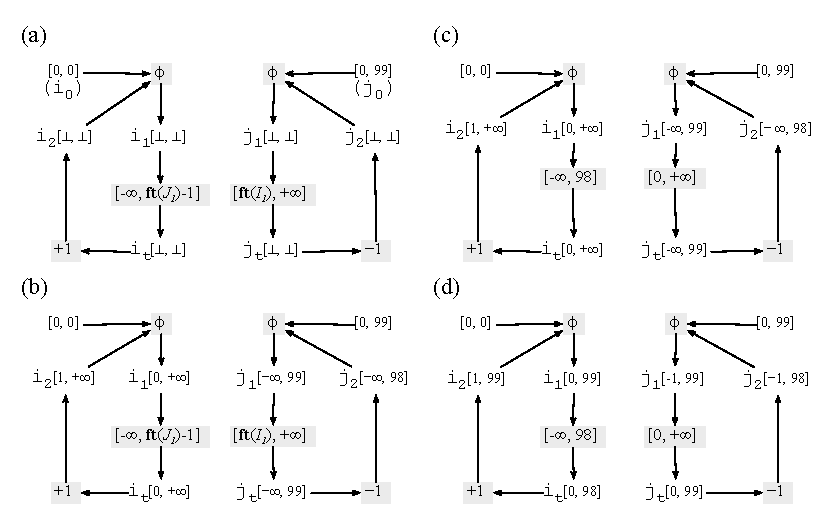
\includegraphics[width=\textwidth]{images/ex_partition_grow_crop}
\end{center}
\caption{\label{fig:ex_partition_grow_crop}
Four snapshots of the last SCC of Figure~\ref{fig:ex_partition_grow_crop}.
(a) After removing control dependence edges, immediately before applying
Cousot and Cousot's operators.
(b) After running the widening analysis.
(c) After fixing the intersections.
(d) After running the narrowing analysis.}
\end{figure}

%\subsection{Alternative Narrowing Operators}
%\label{sub:alt}
%
%Cousot and Cousot's narrowing operator, given in
%Figure~\ref{fig:crop_analysis} is not guaranteed to find the least fixpoint
%of a system of constraints.
%In order to improve the bounds, trading time for precision, we have
%experimented with two other operators.
%The first, is the evaluation function itself, which is given in
%Figure~\ref{fig:eval_function}.
%By iterating it until reaching a fixpoint, we are guaranteed to find the
%optimal solution to the narrowing analysis.
%However, this approach is not practical, because it is equivalent to
%concretely interpreting the program.
%The second alternative that we have tested consists in applying the
%evaluation function on each constraint at most once per intersection.
%We call this approach {\em depth-first narrowing}, because, starting from
%an intersection we visit every node that might be influenced by it.
%After removing control dependence edges, if we are left with a strongly
%connected component containing only {\em ascencing constraints}, that
%is, constraints that only increase the upper bounds of intervals, then this
%approach is guaranteed to find the least fixpoint.
%The same is true if we have a SCC with only {\em descending constraints}.

\section{Experiments}
\label{sec:exp}

% Absolute Time and complexity
% =============================

%Chart 1: shows complexity of the algorithm, plotting program size and time
% to run the analysis.

%Chart 2: time distribution for SPEC only

% Intra/Inter/Inline comparison
% =============================

% Chart 3: Time comparison between intra, inter and inlining:
% Each bar is inter/intra, or inline/intra
% We want to show that the whole program analysis is fast.

% (I) Chart 4: Precision comparison between intra/inter/inline
% *not for spec*: take five largest of bitwise, stanford and SPEC CINT.
% Add the three geomeans to the chart.

% (I) Chart 5: Same as (4), but this time precision in terms of [c, c], [-, c],
% [+, c], [-, +]. Perhaps take off [-, +]

% Impact of e-SSA form:
% =====================

% Chart 6: time overhead e-SSA. So, for each SPEC 2006, do time e-ssa/time ssa.

% (I) Chart 7: precision with e-SSA form.
% Percentage reduction (bitwidth only) for five largest of bitwise, stanford
% and SPEC CINT.

% Size overhead of different representations
% ==========================================

% Chart 8: Size overhead e-SSA/SSA. SPEC 2006 only.

% Chart 9: Size overhead inline/non-inline. SPEC 2006 only.

% Precision with different number of fixed iterations
% ===================================================

% Chart 10: Run inter + e-SSA with N*|SCC| in fixed update for five largest of
% bitwise, stanford and SPEC CINT.

% Table 1: Structural Properties for SPEC CPU 2006.
% Remember to add %SCC's with just one component.

% Impact of strongly connected components
% =======================================

%In our experiments we have observed that the vast majority of strongly
%connected components that constitute typical dependence graphs contain only
%one element.
%Furthermore, composite components tend to be small.
%Therefore, range analysis admit very fast solution.


\section{Final Considerations}
\label{sec:con}

In this presentation we chose to omit correctness proofs for our algorithms.
For a proof that the widening and the narrowing operators give origin to
approximating sequences, we recommend Cousot and Cousot's work~\cite{Cousot}.
For a proof that the e-SSA form transformation is semantics preserving, we
invite the reader to check a recent report of ours~\cite{XXXX}.
In this work we also show that the results that we obtain via the
sparse analysis are equivalent to the results provided by a dense analysis.
In other words, if the dense analysis tells us that variable $v$ is
associated with the interval range $[l, u]$ at program point $i$, and $v'$
is the new name of $v$, alive at $i$ in the e-SSA form program, then $v'$ is
associated with the interval $[l, u]$ along its entire live range.

Our implementation of the range analysis algorithm described in this paper is
publicly available at \texttt{http://google.code/range-analysis/}.
This repository contains instructions about how to deploy and use our
implementation.
We provide a gallery of examples, including source codes,
CFGs and constraint graphs that we produce for meaningful programs at
\texttt{http://google.code/range-analysis/wiki/gallery}.

\bibliographystyle{plain}
\bibliography{references}

\end{document}
